 % arara: clean: { files: [thesis.aux, thesis.bbl, thesis.blg, thesis.dvi, thesis.fdb_latexmk, thesis.fls, thesis.idx, thesis.ilg, thesis.ind, thesis.lof, thesis.log, thesis.lot, thesis.nlo, thesis.nls, thesis.out, thesis.pdf, thesis.ps, thesis.toc]}
% arara: latex:  { shell: yes }
% arara: bibtex
% arara: nomencl
% arara: latex
% arara: makeindex
% arara: latex:  { shell: yes }
% arara: dvips
% arara: ps2pdf

% ******************************* PhD Thesis Template **************************
% Please have a look at the README.md file for info on how to use the template

\documentclass[a4paper,12pt,times,numbered,print,index]{Classes/PhDThesisPSnPDF}

% ******************************************************************************
% ******************************* Class Options ********************************
% *********************** See README for more details **************************
% ******************************************************************************

% `a4paper'(The University of Cambridge PhD thesis guidelines recommends a page
% size a4 - default option) or `a5paper': A5 Paper size is also allowed as per
% the Cambridge University Engineering Deparment guidelines for PhD thesis
%
% `11pt' or `12pt'(default): Font Size 10pt is NOT recommended by the University
% guidelines
%
% `oneside' or `twoside'(default): Printing double side (twoside) or single
% side.
%
% `print': Use `print' for print version with appropriate margins and page
% layout. Leaving the options field blank will activate Online version.
%
% `index': For index at the end of the thesis
%
% `draft': For draft mode without loading any images (same as draft in book)
%
% `draftmode': Special draft mode with line numbers, images, and water mark with
% timestamp and custom text. Position of the text can also be modified.
%
% `abstract': To generate only the title page and abstract page with
% dissertation title and name, to submit to the Student Registry
%
% `chapter`: This option enables only the specified chapter and it's references
%  Useful for review and corrections.
%
% ************************* Custom Page Margins ********************************
%
% `custommargin`: Use `custommargin' in options to activate custom page margins,
% which can be defined in the preamble.tex. Custom margin will override
% print/online margin setup.
%
% *********************** Choosing the Fonts in Class Options ******************
%
% `times' : Times font with math support. (The Cambridge University guidelines
% recommend using times)
%
% `fourier': Utopia Font with Fourier Math font (Font has to be installed)
%            It's a free font.
%
% `customfont': Use `customfont' option in the document class and load the
% package in the preamble.tex
%
% default or leave empty: `Latin Modern' font will be loaded.
%
% ********************** Choosing the Bibliography style ***********************
%
% `authoryear': For author-year citation eg., Krishna (2013)
%
% `numbered': (Default Option) For numbered and sorted citation e.g., [1,5,2]
%
% `custombib': Define your own bibliography style in the `preamble.tex' file.
%              `\RequirePackage[square, sort, numbers, authoryear]{natbib}'.
%              This can be also used to load biblatex instead of natbib
%              (See Preamble)
%
% **************************** Choosing the Page Style *************************
%
% `default (leave empty)': For Page Numbers in Header (Left Even, Right Odd) and
% Chapter Name in Header (Right Even) and Section Name (Left Odd). Blank Footer.
%
% `PageStyleI': Chapter Name next & Page Number on Even Side (Left Even).
% Section Name & Page Number in Header on Odd Side (Right Odd). Footer is empty.
%
% `PageStyleII': Chapter Name on Even Side (Left Even) in Header. Section Number
% and Section Name in Header on Odd Side (Right Odd). Page numbering in footer


% ********************************** Preamble **********************************
% Preamble: Contains packages and user-defined commands and settings
% ******************************************************************************
% ****************************** Custom Margin *********************************

% Add `custommargin' in the document class options to use this section
% Set {innerside margin / outerside margin / topmargin / bottom margin}  and
% other page dimensions
\ifsetCustomMargin
  \RequirePackage[left=37mm,right=30mm,top=35mm,bottom=30mm]{geometry}
  \setFancyHdr % To apply fancy header after geometry package is loaded
\fi

% *****************************************************************************
% ******************* Fonts (like different typewriter fonts etc.)*************

% Add `customfont' in the document class option to use this section

\ifsetCustomFont
  % Set your custom font here and use `customfont' in options. Leave empty to
  % load computer modern font (default LaTeX font).
  \RequirePackage{helvet}
\fi

% *****************************************************************************
% **************************** Custom Packages ********************************

% ************************* Algorithms and Pseudocode **************************

%\usepackage{algpseudocode}


% ********************Captions and Hyperreferencing / URL **********************

% Captions: This makes captions of figures use a boldfaced small font.
%\RequirePackage[small,bf]{caption}

\RequirePackage[labelsep=space,tableposition=top]{caption}
\renewcommand{\figurename}{Fig.} %to support older versions of captions.sty


% *************************** Graphics and figures *****************************

%\usepackage{rotating}
%\usepackage{wrapfig}

% Uncomment the following two lines to force Latex to place the figure.
% Use [H] when including graphics. Note 'H' instead of 'h'
%\usepackage{float}
%\restylefloat{figure}

% Subcaption package is also available in the sty folder you can use that by
% uncommenting the following line
% This is for people stuck with older versions of texlive
%\usepackage{sty/caption/subcaption}
\usepackage{subcaption}

%added by Ruichen Teng
\usepackage{pdfpages}
%added by Ruichen Teng

% ********************************** Tables ************************************
\usepackage{booktabs} % For professional looking tables
\usepackage{multirow}

%\usepackage{multicol}
%\usepackage{longtable}
%\usepackage{tabularx}


% ***************************** Math and SI Units ******************************

\usepackage{amsfonts}
\usepackage{amsmath}
\usepackage{amssymb}
\usepackage{siunitx} % use this package module for SI units


% ******************************* Line Spacing *********************************

% Choose linespacing as appropriate. Default is one-half line spacing as per the
% University guidelines

% \doublespacing
 \onehalfspacing
% \singlespacing


% ************************ Formatting / Footnote *******************************

% Don't break enumeration (etc.) across pages in an ugly manner (default 10000)
%\clubpenalty=500
%\widowpenalty=500

%\usepackage[perpage]{footmisc} %Range of footnote options


% *****************************************************************************
% *************************** Bibliography  and References ********************

%\usepackage{cleveref} %Referencing without need to explicitly state fig /table

% Add `custombib' in the document class option to use this section
\ifuseCustomBib
   \RequirePackage[square, sort, numbers, authoryear]{natbib} % CustomBib

% If you would like to use biblatex for your reference management, as opposed to the default `natbibpackage` pass the option `custombib` in the document class. Comment out the previous line to make sure you don't load the natbib package. Uncomment the following lines and specify the location of references.bib file

%\RequirePackage[backend=biber, style=numeric-comp, citestyle=numeric, sorting=nty, natbib=true]{biblatex}
%\bibliography{References/references} %Location of references.bib only for biblatex

\fi

% changes the default name `Bibliography` -> `References'
\renewcommand{\bibname}{References}


% *****************************************************************************
% *************** Changing the Visual Style of Chapter Headings ***************
% This section on visual style is from https://github.com/cambridge/thesis

% Uncomment the section below. Requires titlesec package.

%\RequirePackage{titlesec}
%\newcommand{\PreContentTitleFormat}{\titleformat{\chapter}[display]{\scshape\Large}
%{\Large\filleft{\chaptertitlename} \Huge\thechapter}
%{1ex}{}
%[\vspace{1ex}\titlerule]}
%\newcommand{\ContentTitleFormat}{\titleformat{\chapter}[display]{\scshape\huge}
%{\Large\filleft{\chaptertitlename} \Huge\thechapter}{1ex}
%{\titlerule\vspace{1ex}\filright}
%[\vspace{1ex}\titlerule]}
%\newcommand{\PostContentTitleFormat}{\PreContentTitleFormat}
%\PreContentTitleFormat


% ******************************************************************************
% ************************* User Defined Commands ******************************
% ******************************************************************************

% *********** To change the name of Table of Contents / LOF and LOT ************

%\renewcommand{\contentsname}{My Table of Contents}
%\renewcommand{\listfigurename}{My List of Figures}
%\renewcommand{\listtablename}{My List of Tables}


% ********************** TOC depth and numbering depth *************************

\setcounter{secnumdepth}{2}
\setcounter{tocdepth}{2}


% ******************************* Nomenclature *********************************

% To change the name of the Nomenclature section, uncomment the following line

%\renewcommand{\nomname}{Symbols}


% ********************************* Appendix ***********************************

% The default value of both \appendixtocname and \appendixpagename is `Appendices'. These names can all be changed via:

%\renewcommand{\appendixtocname}{List of appendices}
%\renewcommand{\appendixname}{Appndx}

% ******************************** Draft Mode **********************************

% Uncomment to disable figures in `draftmode'
%\setkeys{Gin}{draft=true}  % set draft to false to enable figures in `draft'

% These options are active only during the draft mode
% Default text is "Draft"
%\SetDraftText{DRAFT}

% Default Watermark location is top. Location (top/bottom)
%\SetDraftWMPosition{bottom}

% Draft Version - default is v1.0
%\SetDraftVersion{v1.1}

% Draft Text grayscale value (should be between 0-black and 1-white)
% Default value is 0.75
%\SetDraftGrayScale{0.8}


%% Todo notes functionality
%% Uncomment the following lines to have todonotes.

%\ifsetDraft
%	\usepackage[colorinlistoftodos]{todonotes}
%	\newcommand{\mynote}[1]{\todo[author=kks32,size=\small,inline,color=green!40]{#1}}
%\else
%	\newcommand{\mynote}[1]{}
%	\newcommand{\listoftodos}{}
%\fi

% Example todo: \mynote{Hey! I have a note}


% ************************ Thesis Information & Meta-data **********************
% Thesis title and author information, refernce file for biblatex
% ************************ Thesis Information & Meta-data **********************
%% The title of the thesis
\title{Information Extraction of biomedical relationships in published colon cancer literature}
%\texorpdfstring is used for PDF metadata. Usage:
%\texorpdfstring{LaTeX_Version}{PDF Version (non-latex)} eg.,
%\texorpdfstring{$sigma$}{sigma}

%% Subtitle (Optional)
%\subtitle{Using the CUED template}

%% The full name of the author
\author{Ruichen Teng}

%% Department (eg. Department of Engineering, Maths, Physics)
\dept{Department of Computing and Information Systems}

%% University and Crest
\university{University of Melbourne}
\crest{
\includegraphics[width=0.25\textwidth]{University_Crest}}

%% You can redefine the submission text:
% Default as per the University guidelines:
% ``This dissertation is submitted for the degree of''
%\renewcommand{\submissiontext}{change the default text here if needed}

%% Full title of the Degree
\degreetitle{Master of Information Technology}

%% College affiliation (optional)
%\college{King's College}

%% Submission date
% Default is set as {\monthname[\the\month]\space\the\year}
%\degreedate{September 2014} 

%% Meta information
\subject{LaTeX} \keywords{{LaTeX} {Master Thesis} {IT} {University of Melbourne}}


% ***************************** Abstract Separate ******************************
% To printout only the titlepage and the abstract with the PhD title and the
% author name for submission to the Student Registry, use the `abstract' option in
% the document class.

\ifdefineAbstract
 \pagestyle{empty}
 \includeonly{Declaration/declaration, Abstract/abstract}
\fi

% ***************************** Chapter Mode ***********************************
% The chapter mode allows user to only print particular chapters with references
% Title, Contents, Frontmatter are disabled by default
% Useful option to review a particular chapter or to send it to supervisior.
% To use choose `chapter' option in the document class

\ifdefineChapter
 \includeonly{Chapter3/chapter3}
\fi

% ******************************** Front Matter ********************************
\begin{document}
%added by Ruichen Teng
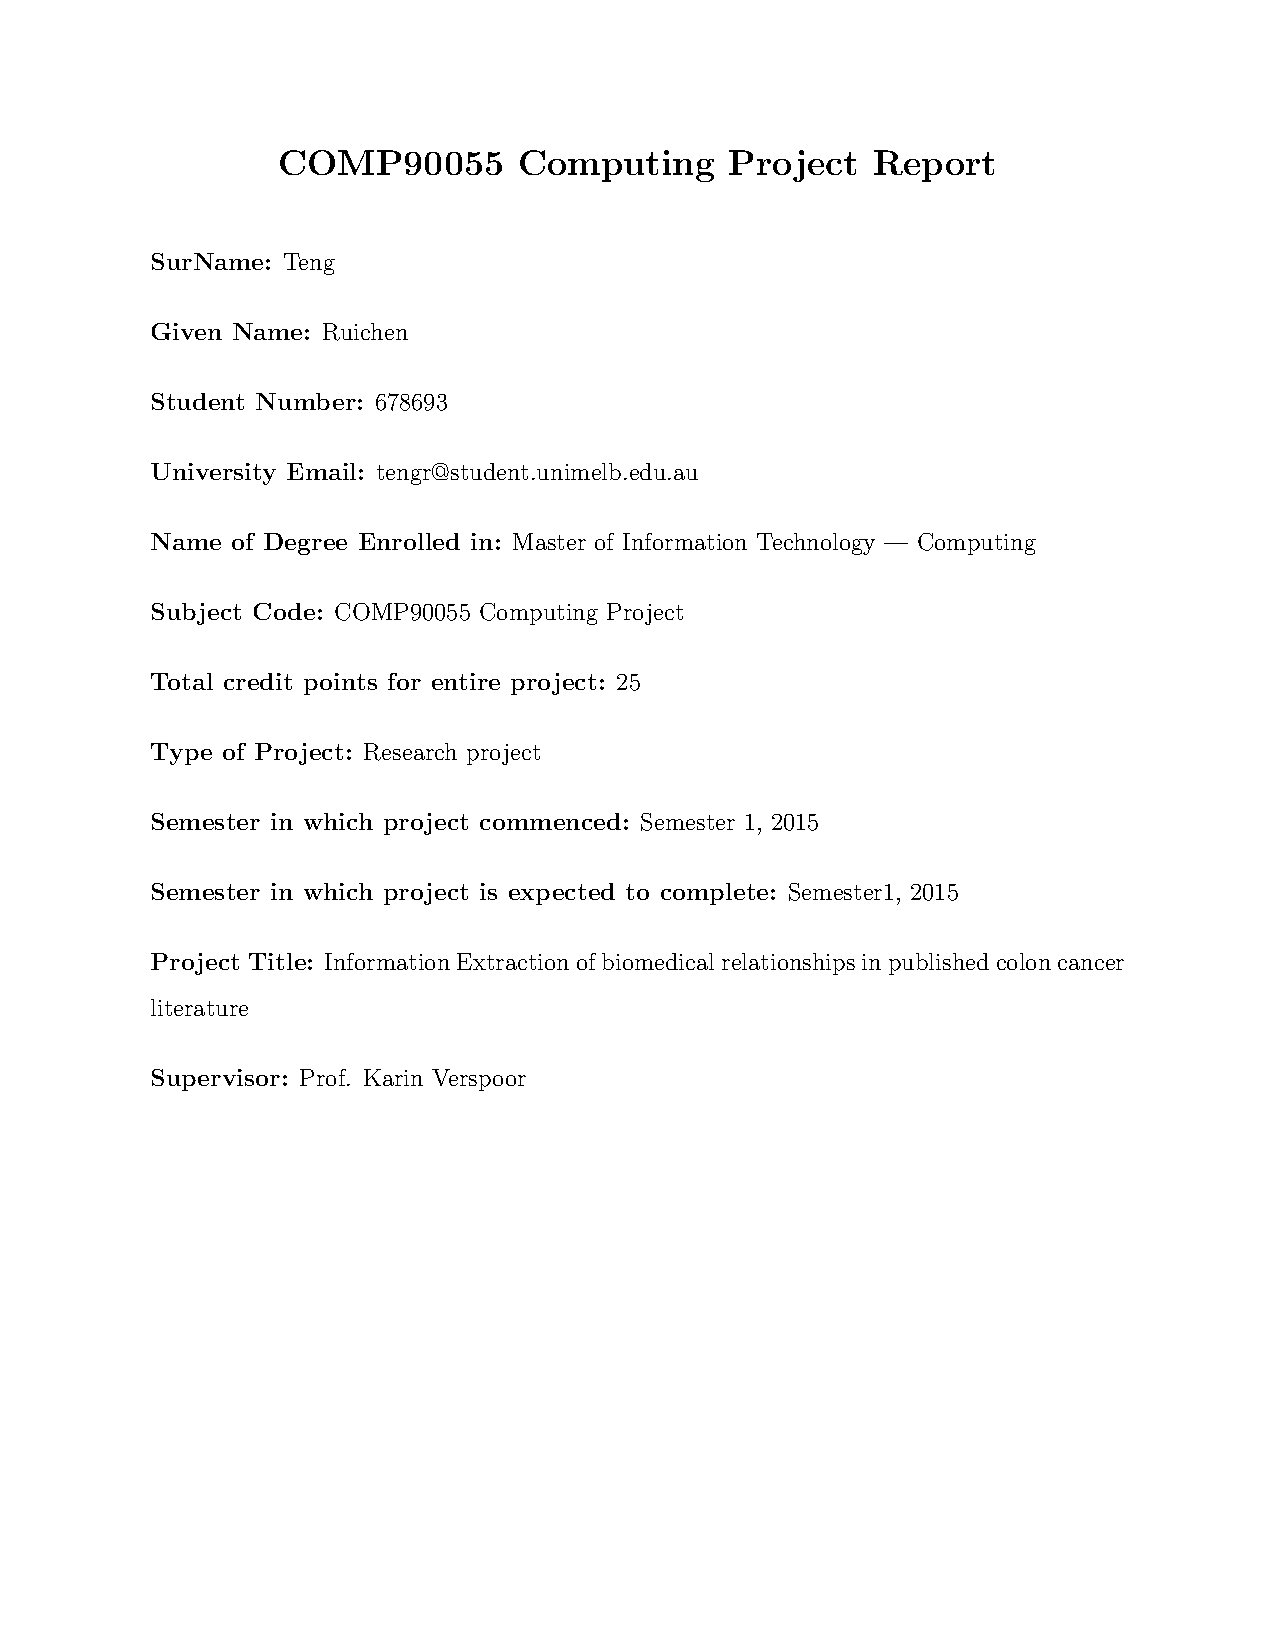
\includepdf[pages=1]{COMP90055_front_page}
%added by Ruichen Teng
\frontmatter

\begin{titlepage}
  \maketitle
\end{titlepage}


% ******************************* Thesis Dedidcation ********************************

\begin{dedication} 

\usefont{T1}{LobsterTwo-LF}{bx}{it}{To my loving parents \dots}

\end{dedication}


% ******************************* Thesis Declaration ***************************

\begin{declaration}
\textit{
I certify that\\ \\
- this thesis does not incorporate without acknowledgement any material previously submitted for a degree or
diploma in any university; and that to the best of my knowledge and belief it does not contain any material
previously published or written by another person where due reference is not made in the text.\\ \\
- the thesis is approximately 6000 words in length (excluding text in images, table, bibliographies and appendices).\\ \\}

%- where necessary I have received clearance for this research from the University's Ethics Committee
%(Approval Number ....) and have submitted all required data to the Department\\ \\

% Author and date will be inserted automatically from thesis.tex \author \degreedate

\end{declaration}


% ************************** Thesis Acknowledgements **************************

\begin{acknowledgements}      
First and foremost, I want to thank my supervisor Prof. Karin Verspoor for the extremely helpful guidance and constant encouragement throughout the duration of this project. Her timely responses have really made this project work. In addition, my gratitude goes to Dr. Haibin Liu and Dr. Andrew MacKinlay for sharing valuable insights into the software system. I would also like to thank Dr. Jeremy Nicholson for chatting with me about NLP research. Finally I would like to thank my friends and family for carrying me through this extremely tough semester.
\end{acknowledgements}

% ************************** Thesis Abstract *****************************
% Use `abstract' as an option in the document class to print only the titlepage and the abstract.
\begin{abstract}
Information extraction (IE) is the task of automatically extracting structured information from unstructured and/or semi-structured machine-readable documents. cite wiki, 
\end{abstract}


% *********************** Adding TOC and List of Figures ***********************

\tableofcontents

\listoffigures

\listoftables

% \printnomencl[space] space can be set as 2em between symbol and description
%\printnomencl[3em]

\printnomencl

% ******************************** Main Matter *********************************
\mainmatter

%added by Ruichen Teng
%*******************************************************************************
%*********************************** First Introduction *****************************
%*******************************************************************************
%\chapter{Introduction}  %Title of the First Introduction
%\chapter*{Introduction}
\chapter{Introduction}  %Title of the First Introduction
%\addcontentsline{tableofcontents}{chapter}{introduction}

\ifpdf
    \graphicspath{{Introduction/Figs/Raster/}{Introduction/Figs/PDF/}{Introduction/Figs/}}
\else
    \graphicspath{{Introduction/Figs/Vector/}{Introduction/Figs/}}
\fi


%********************************** %First Section  **************************************
\section{Motivation}\label{section1.1} %Section - 1.1 
\emph{Text mining} is the process of searching for patterns in natural language text using methods in computer science, linguistics, and statistics. Despite being unstructured and only human-understandable, text is still our primary media for exchange of information\cite{witten2005text}. The prevalence of textual data presents a big challenge to computer-driven natural language understanding. \emph{Information extraction}, in particular, refers to the task of acquiring organized, structured and queryable format of data from the unstructured corpus. \newline\newline
While text mining is widely used in areas like marketing and document verifying, it has received increased attention for its application to biomedical literatures\cite{kim2003genia,ananiadou2006text,krallinger2005text}. This trend stems from the direct need of biomedical workers and researchers to cope with information explosion in their field. For instance, MEDLINE(Medical Literature Analysis and Retrieval System Online), the online database of United States National Library of Medicine, has accumulated nearly 0.8 million citations and 2.7 billion searches in 2014 alone\cite{MEDLINE:2015:Online}, with total citations reaching 25 million. Within these publications there are valuable research results that should add to human knowledge. In the meantime,  our primary knowledge base in life science - the biomedical databases, are still mostly being populated manually by \emph{biocurators} - the ``museum catalogers of the Internet age''\cite{wiki:biocurators}. They are professional scientists who read biomedical articles, record relevant data and organize them according to the biomedical database schema. The sheer volume of publications has made this process increasingly unrealistic\cite{cohen2005survey}.\newline\newline
Not only does data overload make knowledge discovery demanding, it also leads to a decline in literature quality. Nowadays biomedical workers and researchers are more prone to drawing wrong conclusions because they simply can not read all the relevant publications, among which oftentimes contradicting results are reported. Needless to say, we are in desperate need of automatic tools for systematically analyzing documents and extracting information. In fact, it has been argued that text mining is required to improve the coverage of databases\cite{baumgartner2007manual}.


\section{Definitions and Assumptions}
Below are a list of terms which I will use throughout this thesis, detailed examples will be given in the relevant sections, but a general definition is first given here to avoid any confusions that might arise when reading the following paragraphs.
\begin{itemize}
	\item \emph{Relation Extraction:} In general, relation extraction refers two the process of discovering a relationship between entities in text. In the domain of natural language processing, the relation can be semantic, syntactic, etc, with semantic relations being the most important for knowledge discovery. Relations can be unary, binary and complex with complex relations sometimes intermingled with the concept of events, In this project we are mainly concerned with binary relations as shown. Relation extraction is a form of information extraction where the semantic relations between entities are extracted.
	Specifically, in this project we focus on the relation extraction among other informations. Biomedical relations covers a wide range of knowledge in this field.
	\item \emph{Event Extraction:} to be added
\end{itemize}

%********************************** %Second Section  *************************************
\section{Research Question}\label{section1.2}%Section - 1.2
This project looks to investigate the application of information extraction system Approximate Subgraph Matching (ASM)\cite{iu2013approximate},  on relation extraction tasks, specifically regarding the relation extraction on the variome corpus.
In this project we focus on the relation extraction among other informations. Biomedical relations covers a wide range of knowledge in this field. As it turns out, this is not a trivial process, The relation extraction tool has a very promising applications for researchers and medical field workers, pharmaceutical companies, and the general public. 

Relation extraction can be helpful in information search, knowledge discovery and hypothesis generation. 

%********************************** % Third Section  *************************************
\section{Thesis Structure}\label{section1.3} %Section - 1.3
The remainder of the thesis is organized in the following manner. In Chapter 2, we discuss the related work of different algorithms used for relation extraction tasks including pattern-based methods, co-occurrence based methods, rule-based methods and kernel based methods. In Chapter 3, we discuss the Approximate Subgraph Matching(ASM) algorithm in detail and how the system previously used for event extraction in the BioNLP Shared Task 2013 was adapted for the relation extraction task for the Variome Corpus, together with evaluation of extraction results. In Chapter 4, we conclude our work and present future directions.


%*******************************************************************************
%*********************************** First Introduction *****************************
%*******************************************************************************
%\chapter{Introduction}  %Title of the First Introduction
%\chapter*{Introduction}
\chapter{Related Work}  %Title of the First Introduction
%\addcontentsline{tableofcontents}{chapter}{introduction}

\ifpdf
    \graphicspath{{RelatedWork/Figs/Raster/}{RelatedWork/Figs/PDF/}{Introduction/Figs/}}
\else
    \graphicspath{{RelatedWork/Figs/Vector/}{RelatedWork/Figs/}}
\fi

%********************************** %First Section  **************************************
\section{Motivation} %Section - 1.1 

Lorem Ipsum is simply dummy text of the printing and typesetting industry (see 
Section~\ref{section1.3}). Lorem Ipsum~\citep{Aup91} has been the industry's 
standard dummy text ever since the 1500s, when an unknown printer took a galley 
of type and scrambled it to make a type specimen book. It has survived not only 
five centuries, but also the leap into electronic typesetting, remaining 
essentially unchanged. It was popularised in the 1960s with the release of 
Letraset sheets containing Lorem Ipsum passages, and more recently with desktop 
publishing software like Aldus PageMaker including versions of Lorem 
Ipsum~\citep{AAB95,Con90,LM65}.

The most famous equation in the world: $E^2 = (m_0c^2)^2 + (pc)^2$, which is 
known as the \textbf{energy-mass-momentum} relation as an in-line equation.

A {\em \LaTeX{} class file}\index{\LaTeX{} class file@LaTeX class file} is a file, which holds style information for a particular \LaTeX{}.


\begin{align}
CIF: \hspace*{5mm}F_0^j(a) = \frac{1}{2\pi \iota} \oint_{\gamma} \frac{F_0^j(z)}{z - a} dz
\end{align}

\nomenclature[z-cif]{$CIF$}{Cauchy's Integral Formula}                                % first letter Z is for Acronyms 
\nomenclature[a-F]{$F$}{complex function}                                                   % first letter A is for Roman symbols
\nomenclature[g-p]{$\pi$}{ $\simeq 3.14\ldots$}                                             % first letter G is for Greek Symbols
\nomenclature[g-i]{$\iota$}{unit imaginary number $\sqrt{-1}$}                      % first letter G is for Greek Symbols
\nomenclature[g-g]{$\gamma$}{a simply closed curve on a complex plane}  % first letter G is for Greek Symbols
\nomenclature[x-i]{$\oint_\gamma$}{integration around a curve $\gamma$} % first letter X is for Other Symbols
\nomenclature[r-j]{$j$}{superscript index}                                                       % first letter R is for superscripts
\nomenclature[s-0]{$0$}{subscript index}                                                        % first letter S is for subscripts


%********************************** %Second Section  *************************************
\section{Why do we use loren ipsum?} %Section - 1.2


It is a long established fact that a reader will be distracted by the readable content of a page when looking at its layout. The point of using Lorem Ipsum is that it has a more-or-less normal distribution of letters, as opposed to using `Content here, content here', making it look like readable English. Many desktop publishing packages and web page editors now use Lorem Ipsum as their default model text, and a search for `lorem ipsum' will uncover many web sites still in their infancy. Various versions have evolved over the years, sometimes by accident, sometimes on purpose (injected humour and the like).

%********************************** % Third Section  *************************************
\section{Where does it come from?}  %Section - 1.3 
\label{section1.3}

Contrary to popular belief, Lorem Ipsum is not simply random text. It has roots in a piece of classical Latin literature from 45 BC, making it over 2000 years old. Richard McClintock, a Latin professor at Hampden-Sydney College in Virginia, looked up one of the more obscure Latin words, consectetur, from a Lorem Ipsum passage, and going through the cites of the word in classical literature, discovered the undoubtable source. Lorem Ipsum comes from sections 1.10.32 and 1.10.33 of "de Finibus Bonorum et Malorum" (The Extremes of Good and Evil) by Cicero, written in 45 BC. This book is a treatise on the theory of ethics, very popular during the Renaissance. The first line of Lorem Ipsum, "Lorem ipsum dolor sit amet..", comes from a line in section 1.10.32.

The standard chunk of Lorem Ipsum used since the 1500s is reproduced below for those interested. Sections 1.10.32 and 1.10.33 from ``de Finibus Bonorum et Malorum" by Cicero are also reproduced in their exact original form, accompanied by English versions from the 1914 translation by H. Rackham

``Lorem ipsum dolor sit amet, consectetur adipisicing elit, sed do eiusmod tempor incididunt ut labore et dolore magna aliqua. Ut enim ad minim veniam, quis nostrud exercitation ullamco laboris nisi ut aliquip ex ea commodo consequat. Duis aute irure dolor in reprehenderit in voluptate velit esse cillum dolore eu fugiat nulla pariatur. Excepteur sint occaecat cupidatat non proident, sunt in culpa qui officia deserunt mollit anim id est laborum."

Section 1.10.32 of ``de Finibus Bonorum et Malorum", written by Cicero in 45 BC: ``Sed ut perspiciatis unde omnis iste natus error sit voluptatem accusantium doloremque laudantium, totam rem aperiam, eaque ipsa quae ab illo inventore veritatis et quasi architecto beatae vitae dicta sunt explicabo. Nemo enim ipsam voluptatem quia voluptas sit aspernatur aut odit aut fugit, sed quia consequuntur magni dolores eos qui ratione voluptatem sequi nesciunt. Neque porro quisquam est, qui dolorem ipsum quia dolor sit amet, consectetur, adipisci velit, sed quia non numquam eius modi tempora incidunt ut labore et dolore magnam aliquam quaerat voluptatem. Ut enim ad minima veniam, quis nostrum exercitationem ullam corporis suscipit laboriosam, nisi ut aliquid ex ea commodi consequatur? Quis autem vel eum iure reprehenderit qui in ea voluptate velit esse quam nihil molestiae consequatur, vel illum qui dolorem eum fugiat quo voluptas nulla pariatur?"

1914 translation by H. Rackham: ``But I must explain to you how all this mistaken idea of denouncing pleasure and praising pain was born and I will give you a complete account of the system, and expound the actual teachings of the great explorer of the truth, the master-builder of human happiness. No one rejects, dislikes, or avoids pleasure itself, because it is pleasure, but because those who do not know how to pursue pleasure rationally encounter consequences that are extremely painful. Nor again is there anyone who loves or pursues or desires to obtain pain of itself, because it is pain, but because occasionally circumstances occur in which toil and pain can procure him some great pleasure. To take a trivial example, which of us ever undertakes laborious physical exercise, except to obtain some advantage from it? But who has any right to find fault with a man who chooses to enjoy a pleasure that has no annoying consequences, or one who avoids a pain that produces no resultant pleasure?"

Section 1.10.33 of ``de Finibus Bonorum et Malorum", written by Cicero in 45 BC: ``At vero eos et accusamus et iusto odio dignissimos ducimus qui blanditiis praesentium voluptatum deleniti atque corrupti quos dolores et quas molestias excepturi sint occaecati cupiditate non provident, similique sunt in culpa qui officia deserunt mollitia animi, id est laborum et dolorum fuga. Et harum quidem rerum facilis est et expedita distinctio. Nam libero tempore, cum soluta nobis est eligendi optio cumque nihil impedit quo minus id quod maxime placeat facere possimus, omnis voluptas assumenda est, omnis dolor repellendus. Temporibus autem quibusdam et aut officiis debitis aut rerum necessitatibus saepe eveniet ut et voluptates repudiandae sint et molestiae non recusandae. Itaque earum rerum hic tenetur a sapiente delectus, ut aut reiciendis voluptatibus maiores alias consequatur aut perferendis doloribus asperiores repellat."

1914 translation by H. Rackham: ``On the other hand, we denounce with righteous indignation and dislike men who are so beguiled and demoralized by the charms of pleasure of the moment, so blinded by desire, that they cannot foresee the pain and trouble that are bound to ensue; and equal blame belongs to those who fail in their duty through weakness of will, which is the same as saying through shrinking from toil and pain. These cases are perfectly simple and easy to distinguish. In a free hour, when our power of choice is untrammelled and when nothing prevents our being able to do what we like best, every pleasure is to be welcomed and every pain avoided. But in certain circumstances and owing to the claims of duty or the obligations of business it will frequently occur that pleasures have to be repudiated and annoyances accepted. The wise man therefore always holds in these matters to this principle of selection: he rejects pleasures to secure other greater pleasures, or else he endures pains to avoid worse pains."

%*******************************************************************************
%*********************************** First Introduction *****************************
%*******************************************************************************
%\chapter{Introduction}  %Title of the First Introduction
%\chapter*{Introduction}
\chapter{Project Work}  %Title of the First Introduction
%\addcontentsline{tableofcontents}{chapter}{introduction}

\ifpdf
    \graphicspath{{Core/Figs/Raster/}{Core/Figs/PDF/}{Core/Figs/}}
\else
    \graphicspath{{Core/Figs/Vector/}{Core/Figs/}}
\fi

%********************************** %First Section  **************************************
\section{Data Collection} %Section - 1.1 
Our dataset is the Variome Corpus\cite{verspoor2013annotating}, which is openly accessible. \footnote{\href{http://www.opennicta.com.au/home/health/variome}\url{http://www.opennicta.com.au/home/health/variome}} \citet{verspoor2013annotating} gave a detailed illustration of the document selection and annotation process. I will summarize the main points here.\newline\newline
A major part of the current biomedical research lies in understanding the relations between human genetic variation and disease phenotypes. The \emph{Human Variome Project}, or \emph{HVP}, is a global initiative to collect all genetic variation information affecting human health\cite{ring2006human}. In particular, it acts as a liaison between individuals and organizations to integrate the genetic variants into databases that are open to the general public\cite{verspoor2013annotating}. The \emph{International Society for Gastrointestinal Hereditary Tumours (InSiGHT)}, is an international organization which aims to benefit patients with hereditary gastrointestinal(GI) tumours by research, education and personal assistance. In 2008, InSiGHT and HVP began a collaboration which propels InSiGHT to refine its process in the integration and interpretation of genetic variants. Consequently, a substantial effort was made to understand the mutation of mismatch repair(MMR) genes, the cause of Lynch Syndrome - one of the main syndromes of GI cancer\cite{silva2009mismatch}. A total of 10 full-text articles were selected from PubMed Central\textregistered  by searching the common Lynch syndrome genes. These documents cover inherited colon cancer as well as certain other cancers. The annotation schema, also known as the Variome Annotation Schema\cite{verspoor2013annotating}, include 11 entity types and 13 relation types, as can be seen in the table \ref{table:Variome_Relations}.\newline \newline
\begin{table}[h]
	\caption{Variome Relation Types}
	\centering
	\label{table:Variome_Relations}
	\begin{tabular}{|c | c |c  |}
		\hline 
		{Relation Type} 
		& Entity1 & Entity2\\ 
		\hline
		relatedTo  & mutation & disease \\
		relatedTo & disease & gene\\
		relatedTo & disease & body-part\\
		\hline 
		has     & gene & mutation\\
		has     & mutation & size\\
		has     & disease & characteristic\\
		has     & cohort-patient & age\\
		has     & cohort-patient & characteristic\\
		has     & cohort-patient & disease\\
		has     & cohort-patient & ethnicity\\
		has     & cohort-patient & gender\\
		has     & cohort-patient & mutation\\
		has     & cohort-patient & size \\
		\hline 
	\end{tabular}
\end{table}
In short, the annotation and selection of corpus is inspired by the needs of inSIGHT database, but intended for broader applications. In particular, the annotations are done by two human annotators. As suggested in \cite{verspoor2013annotating}, occasional annotation disagreement has been resolved and the result is merged into a single corpus. Thus in this relation extraction task here, we refer to the manual annotations as the gold standard. 
\section{Dependency Graph and Shortest Path}
	\begin{figure}[h]
		\centering
			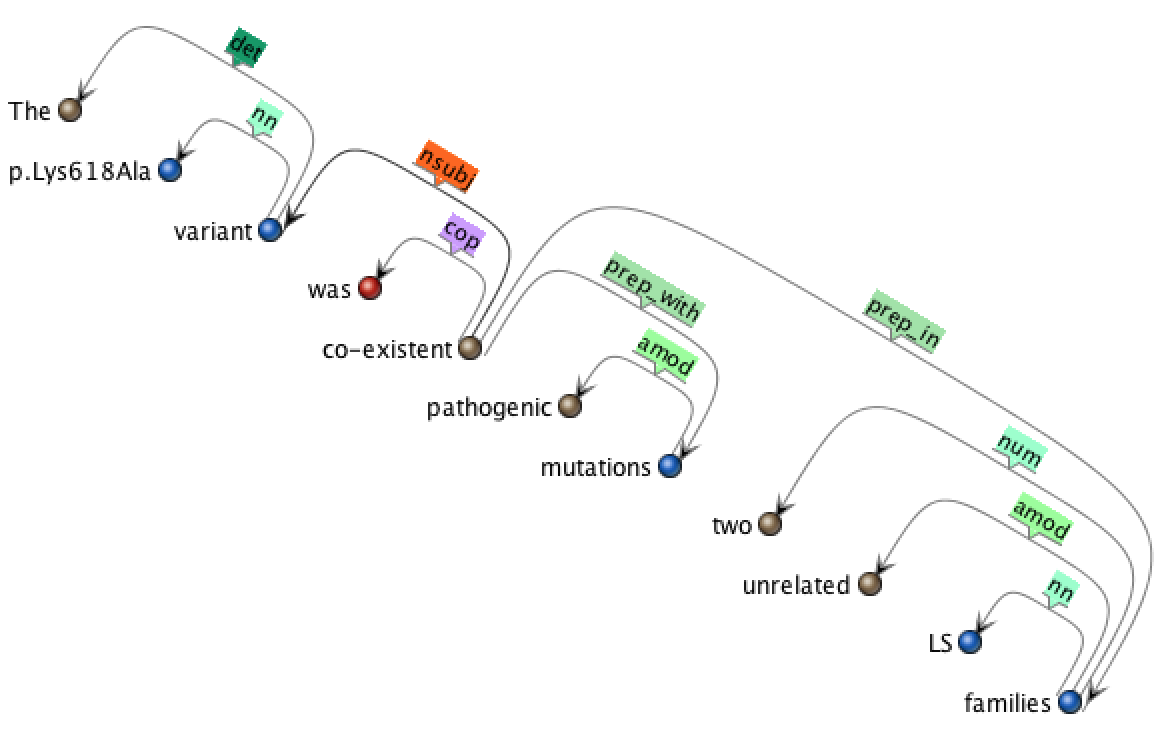
\includegraphics[width=\textwidth]{Dependency_Graph}
			\caption{Dependency Graph of `` The p.Lys618Ala variant was co-existent with pathogenic mutations in two unrelated LS families.''}
			\label{fig:Dependency_Graph}   
	\end{figure}
The dependency graph of a sentence is a directed graph, where nodes represent sentence tokens, and edges indicate their semantic relations. Figure \ref{fig:Dependency_Graph} shows the dependency graph of the sentence \emph{`` The p.Lys618Ala variant was co-existent with pathogenic mutations in two unrelated LS families.''} generated by the Stanford Parser. Such a graph preserves the rich semantic structure of a sentence, and has been widely regarded as an informative way of presenting a sentence. A detailed explanation of the relative constituents in the graph can be found in \cite{de2008stanford}. However, the point is to transfer only human-readable sentences to a computer-understandable data structure. The general idea would be to feed this graph into a learning algorithm and classify relations based on similarity to the sentence graph in the training set. Different approaches exist for this process. Turku Event Extraction System (TEES)\footnote{\href{https://github.com/jbjorne/TEES}https://github.com/jbjorne/TEES}, for instance, engineers a feature vector which consists of token features(part-of-speech tags and character constituents for each word), sentence features(bag-of-words counts), and graph-based features(dependency path represented as N-grams) and builds a multi-class SVM model with the feature vector\cite{bjorne2011generalizing}. In this project, we decide to use the \emph{Shortest Path Hypothesis}\cite{bunescu2005shortest}, namely the heuristic that the relation between two entities in a sentence can be distilled from the shortest path between these entities in the undirected version of the sentence dependency graph. This effectively reduces the burden of feature engineering\cite{liu2013approximate}, but it also calls for high-quality training data. We believe that with effective parameter tuning and clever graph matching techniques, the shortest path can be a single standalone feature for a relation between two entities.
\section{Approximate Subgraph Matching Algorithm}
\textbf{Disclaimer: As the Approximate Subgraph Matching system was originally developed for event extraction, it is more convenient to refer to the system as being learning ``events''. By nature events are nothing more than complex relations between entities, which is exactly the rationale behind adapting such an event extraction system for relations extraction tasks. What was later done in the adaptation process was treating relation as a type of ``event''. In this section, ``relations'' and ``events'' are used (somewhat) interchangeably. }\newline\newline
The Approximate Subgraph Matching framework, proposed by \citet{liu2013approximate} has the following work flow:
\subsection{Prepossessing}
As mentioned in section \ref{2.1}, in order to separate Named Entity Recognition from the Relation Extraction task, the named entity annotations are provided in training, development and test sets. The sentences are identified by the JULIE Sentence Boundary Detector\cite{tomanek2007sentence}, and parsed with the \emph{clearnlp} parser \footnote{\href{https://code.google.com/p/clearnlp/}https://code.google.com/p/clearnlp/}\cite{choi2013transition}. The model for dependency parsing and part-of-speech tagging is trained on the CRAFT corpus \cite{verspoor2012corpus}.
\subsection{Rule Learning}
	\begin{figure}[h]
		\centering
		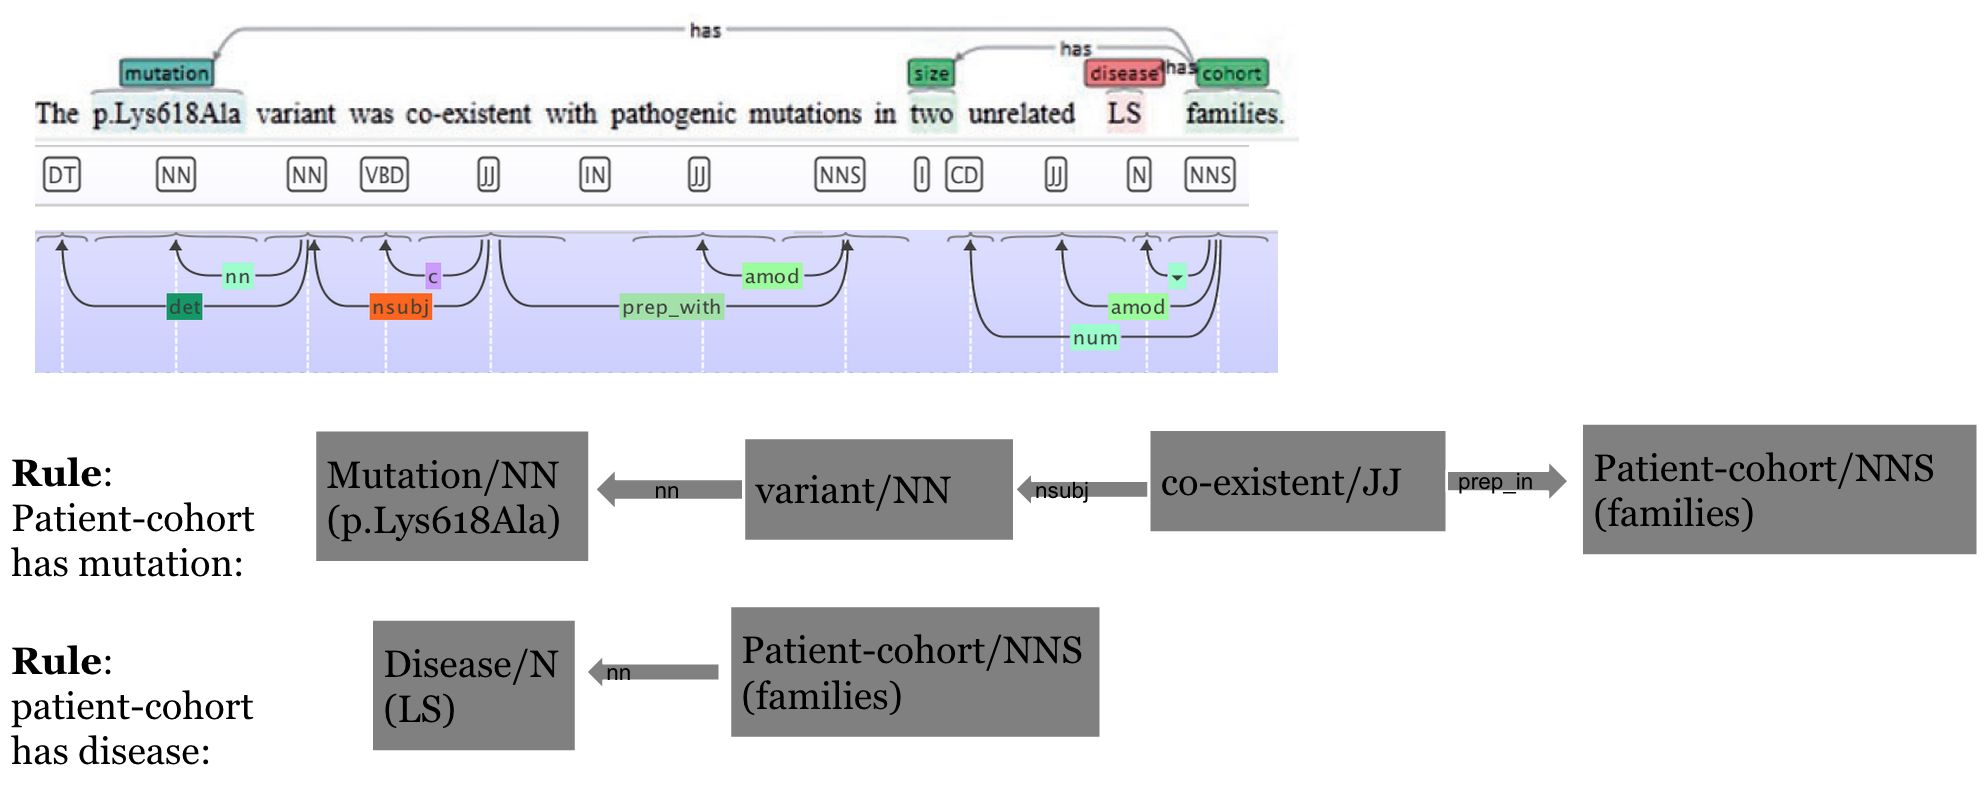
\includegraphics[width=\textwidth]{Rule}
		\caption{Rules learned for `` The p.Lys618Ala variant was co-existent with pathogenic mutations in two unrelated LS families.''}
		\label{fig:Rule}   
	\end{figure}
For each annotated sentence in the training set, a dependency graph is generated and the nodes representing entities are marked. The entity tokens are then replaced with their entity types, such that the rules learned are about an the generic entity types (e.g. gene mutation) instead of specific entities (e.g. p.Lys618Ala), so that our model has a better ability to generalize as we might not see the specific entities again in the test set. Next, the graph is transformed to its undirected version and the shortest path between entities are found with Dijkstra algorithm. This path is leaned as a rule associated with the event type in the annotation as a rule corresponding to that event type. Figure \ref{fig:Rule} gives an example of the learned rules for sentence \emph{`` The p.Lys618Ala variant was co-existent with pathogenic mutations in two unrelated LS families.''} This kind of instance-based learning can be effective provided there is enough training data\cite{alpaydin2014introduction}. A set of rules would then be learned for each event type, representing the graph patterns that indicating a specific type of event. 
\subsection{Sentence Matching}
The rules generated from the previous step could, in theory, be used to match sentences. For each sentence in the test set, a dependency graph can be generated together with the entity annotations(these are provided, as discussed). The graph can be searched exhaustively looking at the path(s) between each entity tokens, for an exact match with one or more rules within the rule set. This step is know as searching for exact subgraph isomorphism. Figure \ref{fig:ESM} gives an example of Exact Subgraph Matching(ESM).\newline\newline
\begin{figure}[h]
	\centering
	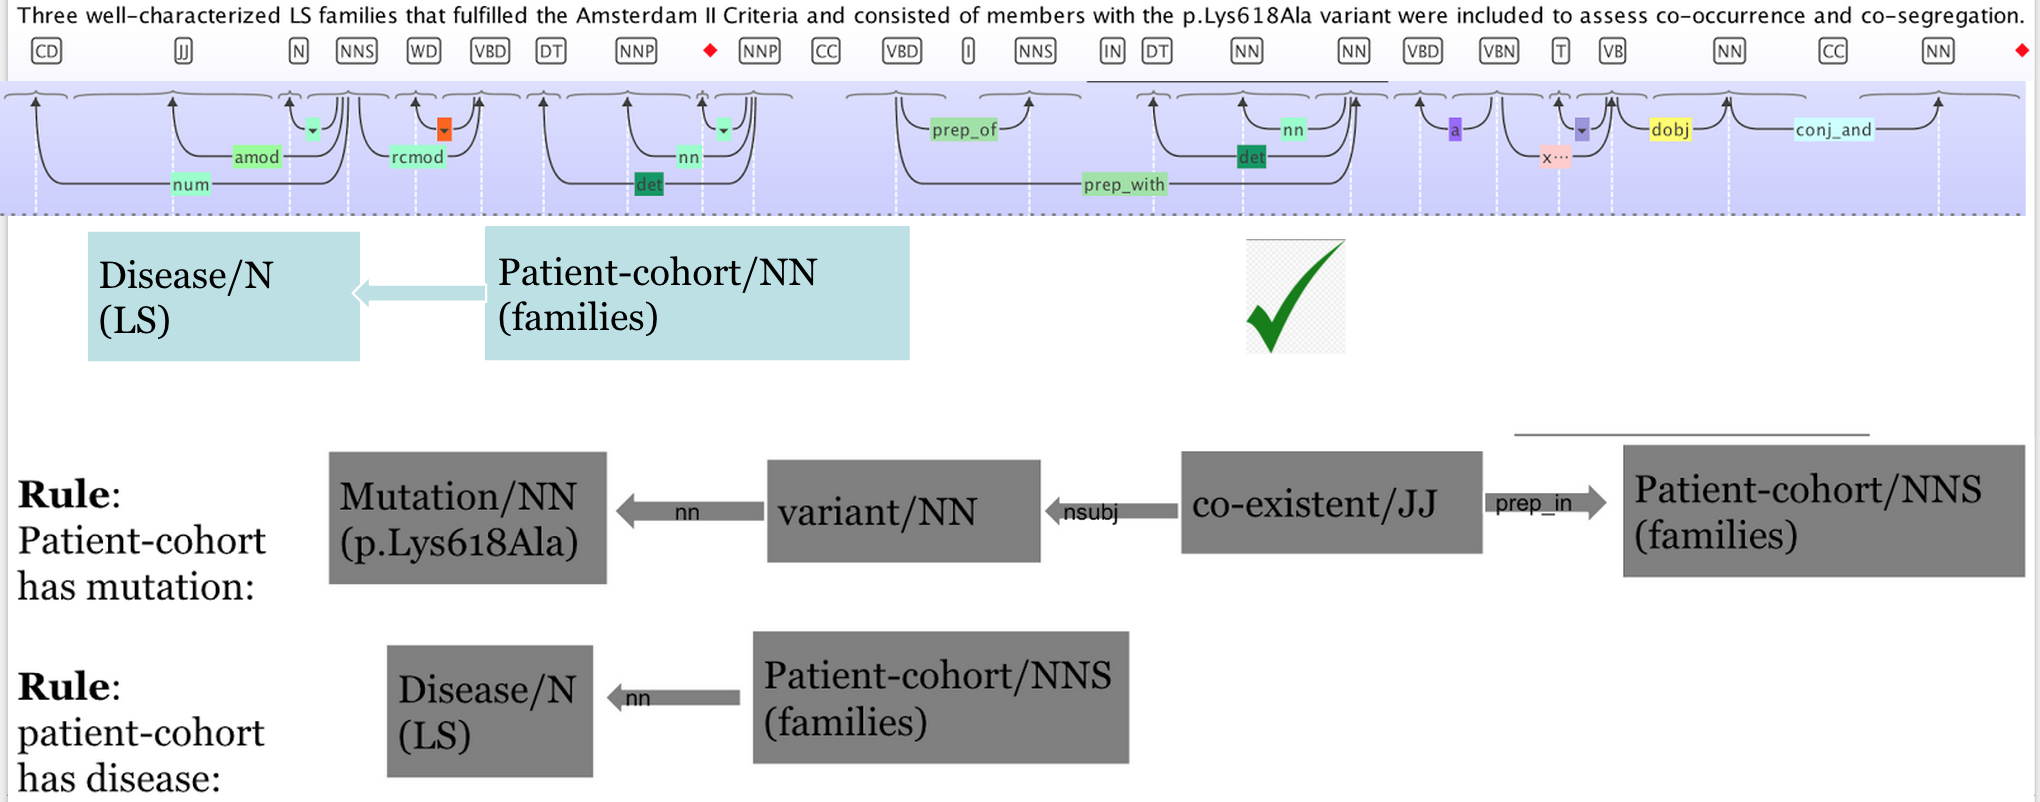
\includegraphics[width=\textwidth]{ESM}
	\caption{Exact Subgraph Matching}
	\label{fig:ESM}   
\end{figure}
However, the above-mentioned matching approach would invariably lead to low recall, as the richness of language can almost always produce slightly different dependency graph structure representing exactly the same events between the same entities. For instance, Figure \ref{fig:ASM} shows a scenario where \emph{patient-cohort has mutation} should be extracted as an event of interest, but there is a slight mismatch in the subgraph patterns. This leads to the rationale behind approximate subgraph matching, which relaxes the matching process and allows for a penalty-based matching. The formula for calculating subgraph distance is: 
\begin{equation}
\begin{split}
GraphDist(SentenceGraph, RuleGraph) = \\
w1 \times structDist(SentenceGraph, RuleGraph)  +\\ 
w2 \times labelDist(SentenceGraph, RuleGraph)   +\\
w3 \times directionalityDist(SentenceGraph, RuleGraph)\\
\end{split}
\end{equation}
$structDist$ is the structural difference between two subgraphs denoted by the distance between each pair of matched nodes. $labelDist$ and $directionalityDist$ are the difference in edge labels and edge directions respectively\cite{liu2013approximate}.
\begin{figure}[h]
	\centering
	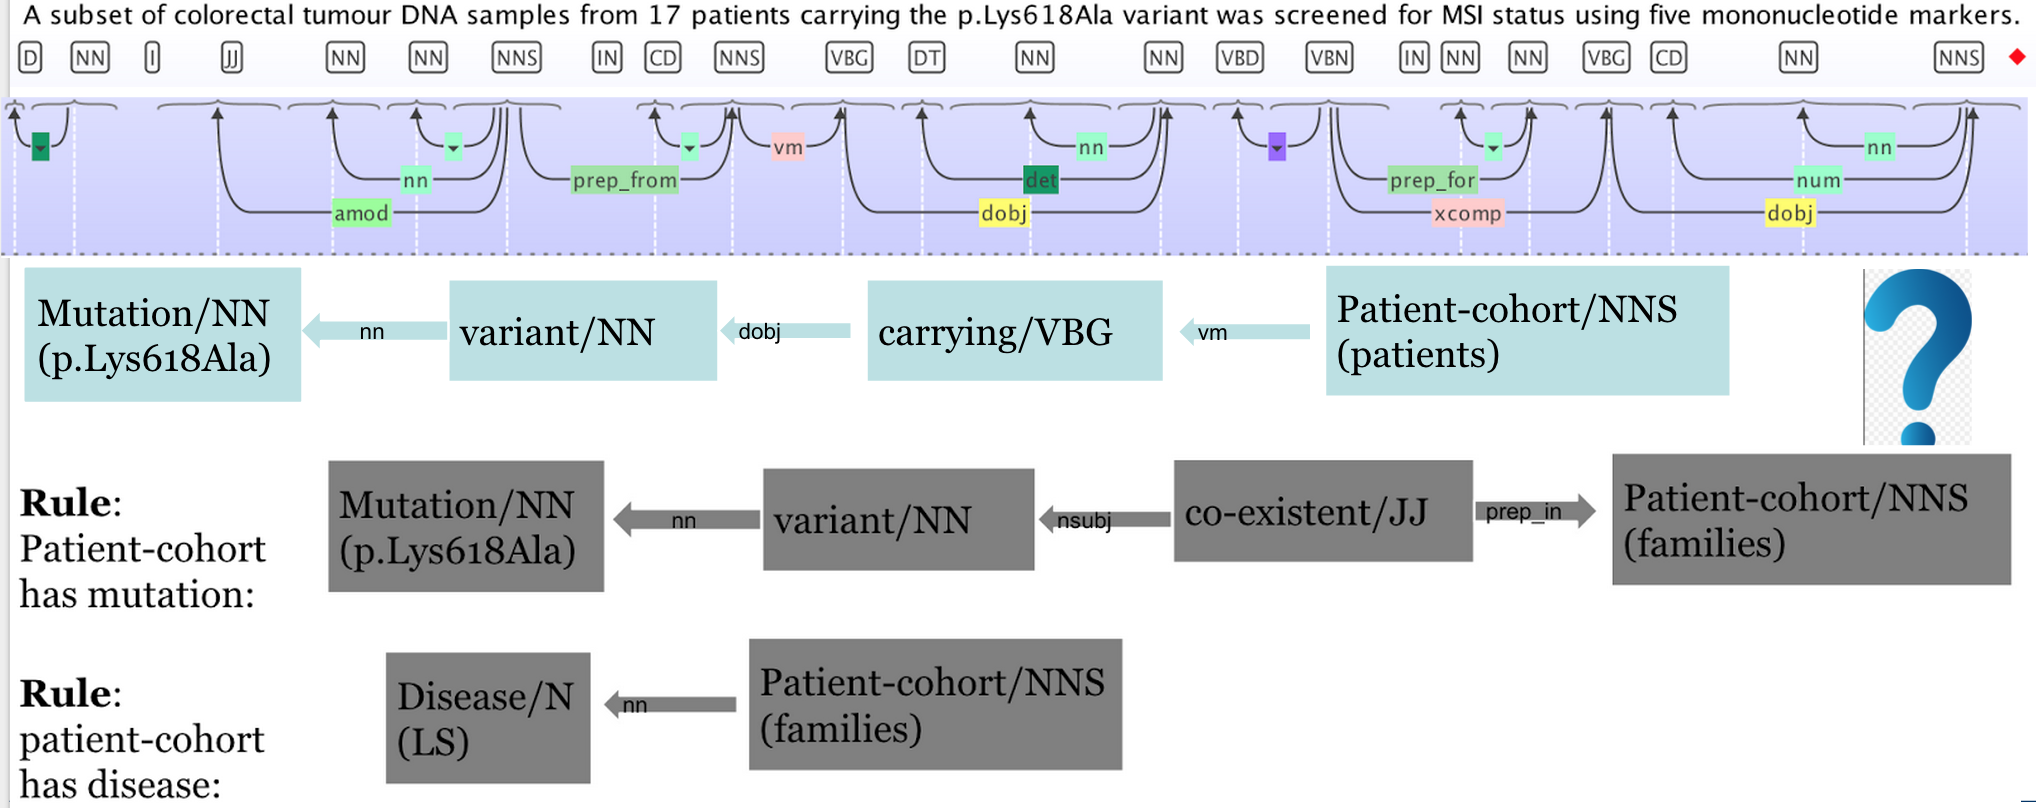
\includegraphics[width=\textwidth]{ASM}
	\caption{Approximate Subgraph Matching}
	\label{fig:ASM}   
\end{figure}
\subsection{Rule Optimization}
To avoid learning the idiosyncrasies in the training data, an iterative rule set optimization process is executed. After the initial learning phase, each rule in the rule set is tested first on the training data to see if it get produce accurate enough predictions (above 0.25). The low performing rules are discarded as a consequence.   
\section{System Adaptation}
\begin{figure}[h]
	\centering
	\begin{subfigure}[b]{0.3\textwidth}
		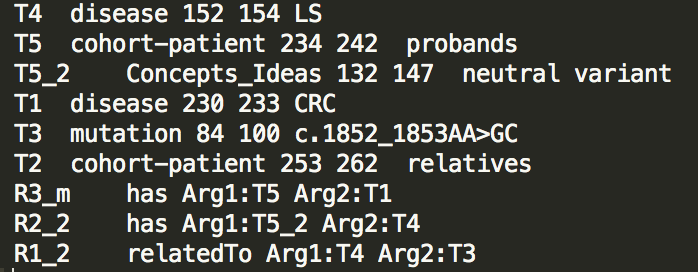
\includegraphics[width=\textwidth]{ann}
		\caption{before	: ann}
		\label{fig:ann}
	\end{subfigure}             
	\vfill
	\begin{subfigure}[b]{0.3\textwidth}
		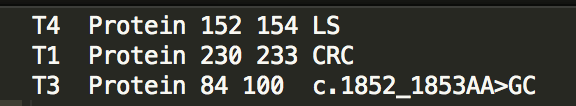
\includegraphics[width=\textwidth]{a1}
		\caption{after: a1}
		\label{fig:a1}   
	\end{subfigure}
	~
	\begin{subfigure}[b]{0.3\textwidth}
		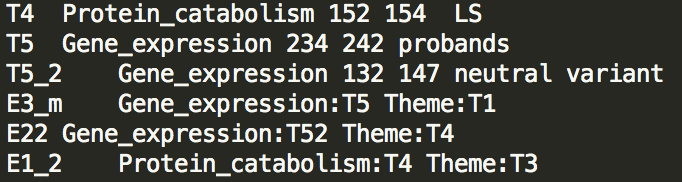
\includegraphics[width=\textwidth]{a2}
		\caption{after: a2}
		\label{fig:a2}   
	\end{subfigure}  
	\caption{Changing Annotation Format}
	\label{fig:annotation_format}
\end{figure}
As mentioned in \ref{section1.3}, the project aims at adapting an existing event extraction system on relation extraction tasks. The existing ASM system was developed for the BioNLP Shared Task 2011 and 2013.\newline\newline \emph{BioNLP shared Task} series is a community-wide text mining challenge specifically for biomedical literatures. The GE task in shared task 2013 aims at retrieving events of the following format: The \emph{.a1} files list all the entities as in Figure \ref{fig:a1}, the \emph{.a2} files list all the event triggers, followed by events as in Figure \ref{fig:a2}. An entity is annotated with its ID, entity type, text offsets, and the textual token. The same goes for triggers. Events are annotated as a relation between the event trigger and one or more entities.\newline\newline
Figure \ref{fig:ann} shows the \emph{Variome Annotation Format}. Different from the shared task, all the annotations would be in one \emph{.ann} file, with entities annotated the same way as in the shared task, and relations similar to events. However, relations do not have triggers at all. This distinction became a major challenge for this project. During the duration of this project, most of my attempts to fully adapt the system to relation extraction tasks have failed. In essence, the differentiation in the retrieval process lies in the event retrieval relies on the detection and prediction of a trigger word, where as the relation extraction does not. \newline\newline
My only attempts that worked was transforming the annotation format of the Variome Corpus to that of the BioNLP Shared Task 2013, such that the original system would not break. The transformation is illustrated in this tables. The "has" relationship is transformed to "gene regulation" event, and "relatedTo" relationship is transformed to "Phosphyrilation" event, with the entity annotation slightly too. The entities would be of type "Protein" instead of the original entity types in the Variome Corpus. \textbf{The major bottleneck for this adaptation work is that the original system includes a hard-coded trigger detection and prediction process.} As for events detecting trigger words such as "activates" for gene expression is an important step for prediction. However, this process is not included at all in the event prediction process and to cope with the original system I had to add "fake triggers" for these events. As a result, the first entity of each event/relation annotation is added as the trigger for the notation. \newline\newline
As shown in Figure \ref{fig:annotation_format}, the original Variome Annotation file (.ann) is splitted into two files(.a1 and .a2), The code checks if the entity exist in any event annotations. If not, the annotation will be ignored such as $T2$. Next the code checks if the annotation is a first argument or second argument. If the annotation is the first argument, it is treated as an event trigger, such as $T4, T5, T5\_2$. The trigger annotations are above the event annotations in the .a2 file where as the other entity annotations are in the .a2 file. 
After this first attempt I had a few better ideas to add fake triggers, the best one being adding the entity types (patient-cohort), with parenthesis directly after the entity tokens and do a binding event. Due to the time constraints and these ideas being essentially fool's gold, I did not implement these ideas.

\section{Results}
\begin{table}[h]
	\caption{Overall Result}
	\centering
	\label{table:overall_result}
	\begin{tabular}{|c | c c |c c c c |}
		\hline 
		{Relation Type} 
		& Gold & Answer  & Match  & Precision & Recall & F1-score\\ 
		\hline
		has  & 1711 & 1310 & 402 & 0.3069 & 0.2350 & 0.2661 \\
		
		relatedTo & 157 & 1498 &  36 & 0.0240 & 0.2293 & 0.0435\\
		\hline 
		TOTAL  & 1868 & 2808 & 438 & 0.1560 & 0.2345 & 0.1874 \\
		\hline 
	\end{tabular}
\end{table}
The overall result of the system is shown in table \ref{table:overall_result}, the main reason the system is not performing well is that it is not predicting the triggers words correctly, because I have chosen to treat entity annotations as triggers. Trigger prediction is usually treated as a classification problem where for every token in the test sentence, a score is assigned for labeling it as trigger for each event type. 

Another important reason is the entity type is quite different from the proteins as proclaimed. 
%*******************************************************************************
%*********************************** First Introduction *****************************
%*******************************************************************************
%\chapter{Introduction}  %Title of the First Introduction
%\chapter*{Introduction}
\chapter{Conclusion}  %Title of the First Introduction
%\addcontentsline{tableofcontents}{chapter}{introduction}

\ifpdf
    \graphicspath{{Conclusion/Figs/Raster/}{Conclusion/Figs/PDF/}{Conclusion/Figs/}}
\else
    \graphicspath{{Conclusion/Figs/Vector/}{Conclusion/Figs/}}
\fi

%********************************** %First Section  **************************************
\section{Conclusion} %Section - 1.1 	
We have explored the possibility of adapting an event-extraction system in relation extraction tasks for the Variome Corpus. 

\section{Contributions}
The contributions of the research in this thesis are as follows:
\begin{itemize}
	\item \emph{The first attempt to use the system outside original system developers.} While this may seem like an easy task, a lot of the time for this project has been devoted to resolving dependencies, and debugging scripts to first have an end-to-end system, even for the original shared task data set.
	\item \emph{The first attempt for literature mining of the Variome Corpus.} To our knowledge, this is the first text mining attempt to the Variome Corpus. 
\end{itemize}
\section{Future Work}
\subsection{Full System Adaptation}
Given the nature of the existing software system, in effect I wrote an adapter for the Variome Corpus, transforming the Variome Corpus Annotations to a format that the ASM system can work with. This is, of course, far from the best solution. However, the ASM system was originally developed solely for an event extraction shared task under time constraints, without much expectation that the system might be adapted on day. As a result, the system annotation format hard-coded in strings and a lot of implicit programming logic such as the involvement of trigger spread out across many different methods, to the extent that all of my efforts to change the code have failed. The main reason for the failure is my inability to detect all the methods and classes where changes should be made, resulting in unexpected system behavior. While is natural and understandable for academic software like this to be one-and-done after use in the shared task, I think it is in the interest of future system users and developers to have a well-documented, adequately extensible system in place, with room for tweaking algorithms and file formats with parameters. Ideally, the shortest path kernel will expose interfaces to users, allowing them to adjust what is happening under the hood with a few parameters. For instance, the existence of trigger should be optional and can be set with a parameter applied to the both the rule learning process and event extraction process. In fact, even in the shared task 2013, the existence of trigger for events like relations or coherence is optional. Next, annotation format should be parametrized, and the system should establish a relationship between user-defined entity and relation types its the entity and relation class. Moreover, the named entity recognition could be a dispatchable unit of the system too, with options to use user-given entities or the output of a named-entity recognizer. A perfect scenario would be one in which the user can input a configuration schema indicating annotation formats, entity types, entity output(whether from the annotation file or from a named entity recognizer), event/relations types and the location of textual data. That way the system can be used for different kinds of tasks, possibly even beyond the domain of biomedical text mining and provide valuable feedback for the plausibility of the approximate subgraph matching paradigm.   
\subsection{Relation Type Fine-Tuning}
Currently, the system only has two relations types, a ``has'' relation and a ``relatedTo'' relation. However, a patient-has-disease relation is semantically quite different from a gene-has-mutation relation, despite both of them being chunked to a single relation type called ``has''. One might be tempted to have fine-grained relation types and incorporate the entity types into the relation, such as a separate ``patient-cohort-has-disease'' and a separate  ``gene-has-mutation'' instead of a ``has'' relation for both. Nevertheless, this would cause the training set to become extremely sparse and the system learning behavior could change drastically. The correlation between granularity of event types and system performance has yet to be explored.  
\subsection{The Parser Effect}
This project uses the exact same preprocessing pipeline as \cite{mackinlay2013extracting}. However, \citet*{mackinlay2013extracting} concluded that changing the parser from the one originally used in \cite{liu2013approximate} has limited recall to an effect that can not be offset by increasing the amount of training data. It was suggested that the longer dependency graph produced by the \emph{clearnlp} parser is harder to generalize. The effect of parser on relation extraction task for the Variome Corpus is yet to be investigated. Again, the parser should be a loosely coupled component of the system too, such that the effect of different dependency parsers can be explored more easily.
\subsection{Parameter Tuning}
Once with an end-to-end system running on the Variome Corpus, the parameters such as subgraph weights, thresholds, rule set optimization aggressiveness need to be tuned for the training set and test parameter tuning on the test set.
\subsection{Combination of Kernels}
A significant limitation of the ASM based approach is the lower recall compared with other systems. 
Successful general literature mining at the semantic level might require a combination of many approaches. The shortest path kernel should be a loosely coupled component of the system and replaceable or by other kernels or a combination of kernels. 
\subsection{The Abstract Effect}
Many earlier biomedical text mining approaches only process abstracts of articles. The rationale is that abstract would contain a summary of the whole article and the important relations that it contains. In the Variome Corpus the full-text articles are splitted into sections such as abstract, introduction, conclusion, etc. With this in mind, one might be careful in how to distribute data for training, development and testing to avoid over-fitting in the future.

%added by Ruichen Teng
%%*******************************************************************************
%*********************************** First Chapter *****************************
%*******************************************************************************

\chapter{Getting started}  %Title of the First Chapter
%\addcontentsline{tableofcontents}{chapter}{Getting started}

\ifpdf
    \graphicspath{{Chapter1/Figs/Raster/}{Chapter1/Figs/PDF/}{Chapter1/Figs/}}
\else
    \graphicspath{{Chapter1/Figs/Vector/}{Chapter1/Figs/}}
\fi


%********************************** %First Section  **************************************
\section{What is loren ipsum? Title with math \texorpdfstring{$\sigma$}{[sigma]}} %Section - 1.1 

Lorem Ipsum is simply dummy text of the printing and typesetting industry (see 
Section~\ref{section1.3}). Lorem Ipsum~\citep{Aup91} has been the industry's 
standard dummy text ever since the 1500s, when an unknown printer took a galley 
of type and scrambled it to make a type specimen book. It has survived not only 
five centuries, but also the leap into electronic typesetting, remaining 
essentially unchanged. It was popularised in the 1960s with the release of 
Letraset sheets containing Lorem Ipsum passages, and more recently with desktop 
publishing software like Aldus PageMaker including versions of Lorem 
Ipsum~\citep{AAB95,Con90,LM65}.

The most famous equation in the world: $E^2 = (m_0c^2)^2 + (pc)^2$, which is 
known as the \textbf{energy-mass-momentum} relation as an in-line equation.

A {\em \LaTeX{} class file}\index{\LaTeX{} class file@LaTeX class file} is a file, which holds style information for a particular \LaTeX{}.


\begin{align}
CIF: \hspace*{5mm}F_0^j(a) = \frac{1}{2\pi \iota} \oint_{\gamma} \frac{F_0^j(z)}{z - a} dz
\end{align}

\nomenclature[z-cif]{$CIF$}{Cauchy's Integral Formula}                                % first letter Z is for Acronyms 
\nomenclature[a-F]{$F$}{complex function}                                                   % first letter A is for Roman symbols
\nomenclature[g-p]{$\pi$}{ $\simeq 3.14\ldots$}                                             % first letter G is for Greek Symbols
\nomenclature[g-i]{$\iota$}{unit imaginary number $\sqrt{-1}$}                      % first letter G is for Greek Symbols
\nomenclature[g-g]{$\gamma$}{a simply closed curve on a complex plane}  % first letter G is for Greek Symbols
\nomenclature[x-i]{$\oint_\gamma$}{integration around a curve $\gamma$} % first letter X is for Other Symbols
\nomenclature[r-j]{$j$}{superscript index}                                                       % first letter R is for superscripts
\nomenclature[s-0]{$0$}{subscript index}                                                        % first letter S is for subscripts


%********************************** %Second Section  *************************************
\section{Why do we use loren ipsum?} %Section - 1.2


It is a long established fact that a reader will be distracted by the readable content of a page when looking at its layout. The point of using Lorem Ipsum is that it has a more-or-less normal distribution of letters, as opposed to using `Content here, content here', making it look like readable English. Many desktop publishing packages and web page editors now use Lorem Ipsum as their default model text, and a search for `lorem ipsum' will uncover many web sites still in their infancy. Various versions have evolved over the years, sometimes by accident, sometimes on purpose (injected humour and the like).

%********************************** % Third Section  *************************************
\section{Where does it come from?}  %Section - 1.3 
\label{section1.3}

Contrary to popular belief, Lorem Ipsum is not simply random text. It has roots in a piece of classical Latin literature from 45 BC, making it over 2000 years old. Richard McClintock, a Latin professor at Hampden-Sydney College in Virginia, looked up one of the more obscure Latin words, consectetur, from a Lorem Ipsum passage, and going through the cites of the word in classical literature, discovered the undoubtable source. Lorem Ipsum comes from sections 1.10.32 and 1.10.33 of "de Finibus Bonorum et Malorum" (The Extremes of Good and Evil) by Cicero, written in 45 BC. This book is a treatise on the theory of ethics, very popular during the Renaissance. The first line of Lorem Ipsum, "Lorem ipsum dolor sit amet..", comes from a line in section 1.10.32.

The standard chunk of Lorem Ipsum used since the 1500s is reproduced below for those interested. Sections 1.10.32 and 1.10.33 from ``de Finibus Bonorum et Malorum" by Cicero are also reproduced in their exact original form, accompanied by English versions from the 1914 translation by H. Rackham

``Lorem ipsum dolor sit amet, consectetur adipisicing elit, sed do eiusmod tempor incididunt ut labore et dolore magna aliqua. Ut enim ad minim veniam, quis nostrud exercitation ullamco laboris nisi ut aliquip ex ea commodo consequat. Duis aute irure dolor in reprehenderit in voluptate velit esse cillum dolore eu fugiat nulla pariatur. Excepteur sint occaecat cupidatat non proident, sunt in culpa qui officia deserunt mollit anim id est laborum."

Section 1.10.32 of ``de Finibus Bonorum et Malorum", written by Cicero in 45 BC: ``Sed ut perspiciatis unde omnis iste natus error sit voluptatem accusantium doloremque laudantium, totam rem aperiam, eaque ipsa quae ab illo inventore veritatis et quasi architecto beatae vitae dicta sunt explicabo. Nemo enim ipsam voluptatem quia voluptas sit aspernatur aut odit aut fugit, sed quia consequuntur magni dolores eos qui ratione voluptatem sequi nesciunt. Neque porro quisquam est, qui dolorem ipsum quia dolor sit amet, consectetur, adipisci velit, sed quia non numquam eius modi tempora incidunt ut labore et dolore magnam aliquam quaerat voluptatem. Ut enim ad minima veniam, quis nostrum exercitationem ullam corporis suscipit laboriosam, nisi ut aliquid ex ea commodi consequatur? Quis autem vel eum iure reprehenderit qui in ea voluptate velit esse quam nihil molestiae consequatur, vel illum qui dolorem eum fugiat quo voluptas nulla pariatur?"

1914 translation by H. Rackham: ``But I must explain to you how all this mistaken idea of denouncing pleasure and praising pain was born and I will give you a complete account of the system, and expound the actual teachings of the great explorer of the truth, the master-builder of human happiness. No one rejects, dislikes, or avoids pleasure itself, because it is pleasure, but because those who do not know how to pursue pleasure rationally encounter consequences that are extremely painful. Nor again is there anyone who loves or pursues or desires to obtain pain of itself, because it is pain, but because occasionally circumstances occur in which toil and pain can procure him some great pleasure. To take a trivial example, which of us ever undertakes laborious physical exercise, except to obtain some advantage from it? But who has any right to find fault with a man who chooses to enjoy a pleasure that has no annoying consequences, or one who avoids a pain that produces no resultant pleasure?"

Section 1.10.33 of ``de Finibus Bonorum et Malorum", written by Cicero in 45 BC: ``At vero eos et accusamus et iusto odio dignissimos ducimus qui blanditiis praesentium voluptatum deleniti atque corrupti quos dolores et quas molestias excepturi sint occaecati cupiditate non provident, similique sunt in culpa qui officia deserunt mollitia animi, id est laborum et dolorum fuga. Et harum quidem rerum facilis est et expedita distinctio. Nam libero tempore, cum soluta nobis est eligendi optio cumque nihil impedit quo minus id quod maxime placeat facere possimus, omnis voluptas assumenda est, omnis dolor repellendus. Temporibus autem quibusdam et aut officiis debitis aut rerum necessitatibus saepe eveniet ut et voluptates repudiandae sint et molestiae non recusandae. Itaque earum rerum hic tenetur a sapiente delectus, ut aut reiciendis voluptatibus maiores alias consequatur aut perferendis doloribus asperiores repellat."

1914 translation by H. Rackham: ``On the other hand, we denounce with righteous indignation and dislike men who are so beguiled and demoralized by the charms of pleasure of the moment, so blinded by desire, that they cannot foresee the pain and trouble that are bound to ensue; and equal blame belongs to those who fail in their duty through weakness of will, which is the same as saying through shrinking from toil and pain. These cases are perfectly simple and easy to distinguish. In a free hour, when our power of choice is untrammelled and when nothing prevents our being able to do what we like best, every pleasure is to be welcomed and every pain avoided. But in certain circumstances and owing to the claims of duty or the obligations of business it will frequently occur that pleasures have to be repudiated and annoyances accepted. The wise man therefore always holds in these matters to this principle of selection: he rejects pleasures to secure other greater pleasures, or else he endures pains to avoid worse pains."

%\include{Chapter2/chapter2}
%\include{Chapter3/chapter3}
%\include{Chapter4/chapter4}
%\include{Chapter5/chapter5}
%\include{Chapter6/chapter6}
%\include{Chapter7/chapter7}



% ********************************** Back Matter *******************************
% Backmatter should be commented out, if you are using appendices after References
%\backmatter

% ********************************** Bibliography ******************************
\begin{spacing}{0.9}

% To use the conventional natbib style referencing
% Bibliography style previews: http://nodonn.tipido.net/bibstyle.php
% Reference styles: http://sites.stat.psu.edu/~surajit/present/bib.htm

\bibliographystyle{apalike}
%\bibliographystyle{plainnat} % use this to have URLs listed in References
\cleardoublepage
\bibliography{References/references} % Path to your References.bib file


% If you would like to use BibLaTeX for your references, pass `custombib' as
% an option in the document class. The location of 'reference.bib' should be
% specified in the preamble.tex file in the custombib section.
% Comment out the lines related to natbib above and uncomment the following line.

%\printbibliography[heading=bibintoc, title={References}]


\end{spacing}

% ********************************** Appendices ********************************

%\begin{appendices} % Using appendices environment for more functunality

%\include{Appendix1/appendix1}
%\include{Appendix2/appendix2}

%\end{appendices}

% *************************************** Index ********************************
%\printthesisindex % If index is present

\end{document}
